\begin{quote}
	\textbf{Abstract:} 
\end{quote}

\section{Introduction}
Continuous technological advancements to high-throughput profiling of single cells
are having profound effects on how researchers can validate biological hypotheses. 
For example, single-cell RNA sequencing (scRNA-seq) directly resulted in the development
of a new type of computational method called trajectory inference (TI). By profiling
the transcriptomics profiles of developing cells, TI methods attempt to reconstruct 
and characterise the underlying dynamic processes \cite{cannoodt_computationalmethodstrajectory_2016}.
While early experimental technologies allowed to profile one single modality (e.g. DNA sequence, 
RNA or protein expression), recent developments permit profiling multiple modalities simultaneously.

An ideal experiment would be able to observe all aspects of a cell, including a full history of its 
molecular states, spatial positions and environmental interactions \cite{stuart_integrativesinglecellanalysis_2019}. 
While this falls outside the reach of current experimental technologies, \textit{in silico} simulations
of single cells would allow developing the next wave of computational techniques
in anticipation of new experimental technologies.

A few generators of scRNA-seq profiles have already been developed (e.g. splatter \cite{zappia_splattersimulationsinglecell_2017}, powsimR \cite{vieth_powsimrpoweranalysis_2017} and PROSSTT \cite{papadopoulos_prossttprobabilisticsimulation_2018}). % BoolODE and dyntoy are also examples.
These can be used to evaluate the performance of computational tools, and to explore their strengths and weaknesses. A limitation of directly simulating a scRNA-seq profile (instead of a single cell) is that extending the simulation to other aspects of the cell -- such as tracking the full history of molecular states -- becomes difficult.

We introduce dyngen, a multi-modality simulator of single cells (Figure \ref{fig:dyngen}).
dyngen was initially developed as part of a comprehensive benchmark of TI methods \cite{saelens_comparisonsinglecelltrajectory_2019} but has since been extended to be applicable in a much broader context.
We demonstrate its flexibility by simulating numerous different types of biological experiments, and using these simulations to develop new benchmarking techniques for computational tools.

\begin{figure}[htb!]
	\centering
	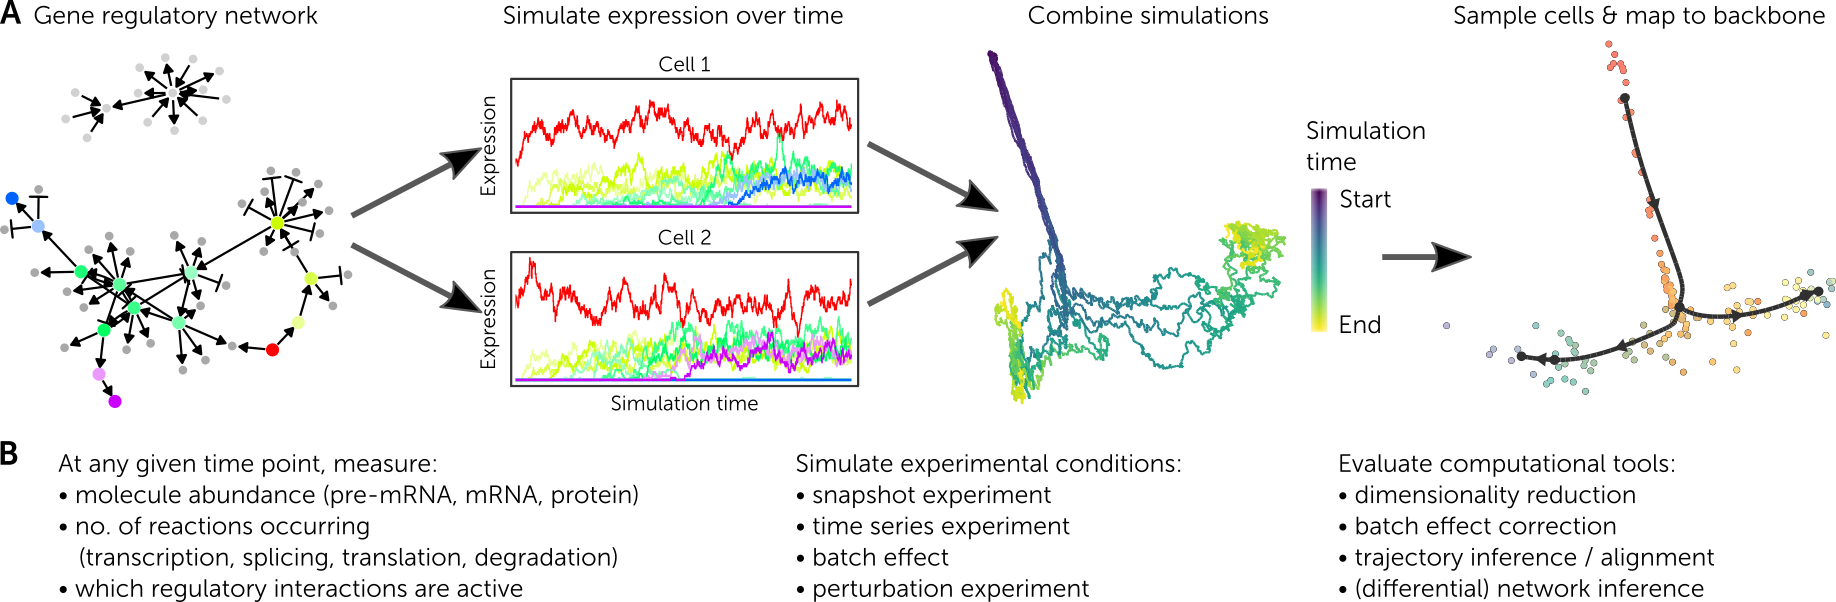
\includegraphics[width=\linewidth]{fig/showcase_3.png} 
	\caption{Showcase of dyngen functionality. \textbf{TODO: change to pdf.} Remove B?} % TODO: update label
	\label{fig:dyngen}
\end{figure}

\section{Results}
dyngen is a simulator for single cells that develop over time. Throughout this section, a simple simulation of a cell undergoing a cyclic process is used to illustrate key strengths of dyngen (Figure \ref{fig:simplecyclic}). This example only comprises of a single cell containing 5 genes, but dyngen can easily scale up to thousands of simulations containing thousands of genes.

\begin{figure}[htb!]
	\centering
	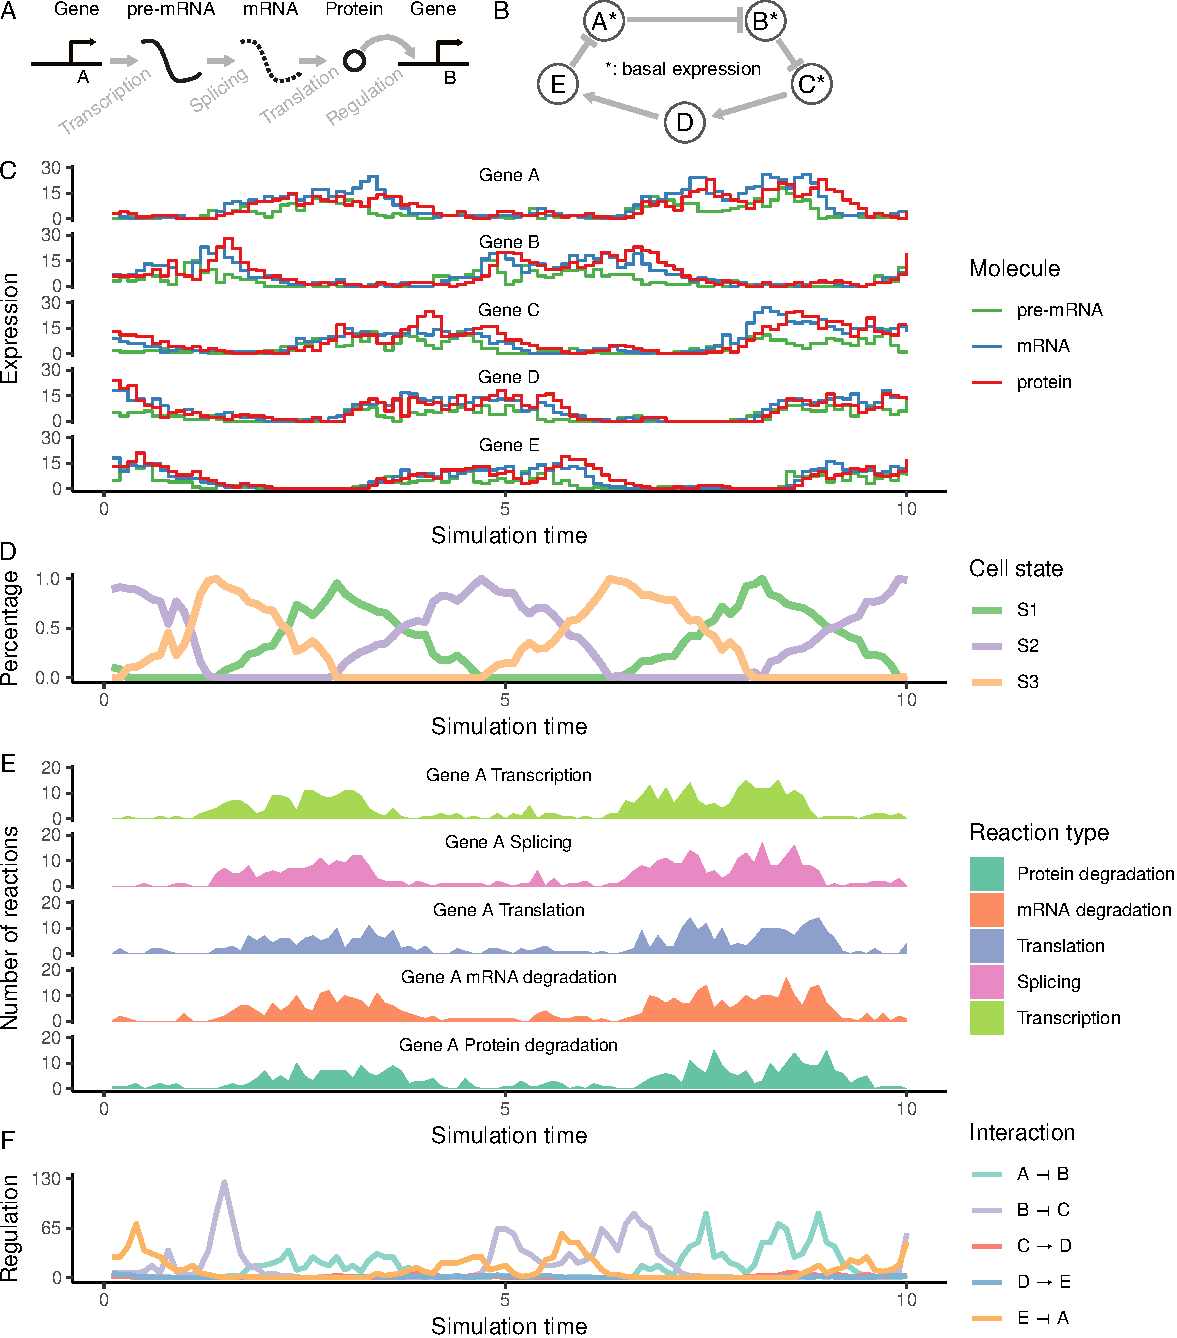
\includegraphics[width=\linewidth]{fig/simplecyclic_edited} 
	\caption{Showcase of dyngen functionality. A time resolution of 0.1 was used, but this can be increased or decreased without effect on performance of the execution of the simulation. \textbf{TODO: perhaps it's better to replace Figure \ref{fig:simplecyclic} with one subfigure for each of the paragraphs in this text.}}
	\label{fig:simplecyclic}
\end{figure}

In dyngen, a cell consists of a set of molecules, the abundance of which are affected by a set of reactions: transcription, splicing, translation, and degradation (Figure \ref{fig:simplecyclic}A). These reactions are determined from a predefined set of gene regulatory interactions (Figure \ref{fig:simplecyclic}B), henceforth referred to as a gene regulatory network (GRN). The likelihood of a reaction occurring at any given point in time is defined by the GRN and by the abundance of molecules involved each reaction.

One of dyngen's main advantages is that through careful engineering of the GRN, different cellular developmental processes can be obtained. Different GRNs can result in branching, converging, cyclic, or even disconnected developmental topologies. Multiple simulations with slightly different GRNs can emulate rewiring events in disease or perturbation experiments. % could use figure; one with GRNs of different topologies, another with rewiring events
Multiple simulations with different initial molecule abundance levels can be used to replicate batch effects. 

Another advantage is that dyngen returns many modalities throughout the whole simulation: molecular abundance, cellular state, number of reaction firings, reaction likelihoods, and regulation activations (Figure \ref{fig:simplecyclic}C--F). These modalities can serve both as input data and ground truth for benchmarking many types of computational approaches. For example, a network inference method could use mRNA abundance and cellular states as inputs, and its output could be benchmarked against the gold standard GRN.

The final main advantage is that by making alterations to the simulation pipeline, multiple types of experiments (sampling technique or profiling technique) can be simulated. By default, dyngen supports snapshot experiments (uniformly sampling from an asynchronous dynamic process) and time-series experiments (sampling cells from different intervals in the simulation). 
It is possible to implement other experimental protocols (which perhaps do not exist in real life), such as sampling the same cell at regular intervals. 

%% TODO: show that dyngen output resembles real data using e.g. countsimQC?

\section{Discussion}
As is, dyngen's single cell simulations can be used to evaluate common single-cell omics computational methods such as clustering, batch correction, trajectory inference and network inference.
However, the combined effect of these advantages results in a framework that is flexible enough to adapt to a broad range of applications. This may include methods that integrate clustering, network inference and trajectory inference. In this respect, dyngen may promote the development of new tools in the single-cell field similarly as other simulators have done in the past \cite{schaffter_genenetweaversilicobenchmark_2011,ewing_combiningtumorgenome_2015}.

Adding batch effects to snapshot simulations of linear (or even branching) trajectories allows evaluating trajectory alignment methods -- which attempt to map two or more trajectories onto each other. Adding perturbations to the GRN allows evaluating the performance of differential network inference methods -- which predict differential regulatory interactions between two or more groups of profiles.  Sampling a cell at a particular time point and once more at a later time point allows evaluating the performance of RNA velocity approaches -- which predict the future state of a cell by looking at differences in pre-mRNA and mRNA abundance levels.

dyngen ultimately also allows anticipating technological developments in single-cell multi-omics. In this way, it is possible to design and evaluate the performance and robustness of new types of computational analyses before experimental data becomes available.
Similarly, it could also be used to compare which experimental technique will likely produce the most accurate result. For example, is it possible to infer directionality of regulatory interactions from snapshot experiments only, or are time series or knockdown experiments a necessity in order to infer high-quality regulatory networks?

Currently, dyngen focuses on simulating cells as standalone entities.
Future developments include extending the framework to simulate multiple cells in a virtual environment. Allowing cells to receive and react to environmental and intercellular stimuli would enable simulating essential cellular processes such as cell division and migration. 
%¡also adding more types of molecules, e.g. protein complex, small rnas, PPI
\section{Methods}

dyngen's approach was inspired by GeneNetWeaver's \cite{schaffter_genenetweaversilicobenchmark_2011} workflow to generate \textit{in silico} bulk profiles for evaluating network inference methods \cite{marbach_wisdomcrowdsrobust_2012}. The workflow to generate \textit{in silico} single cell data consists of six main steps (Figure \ref{fig:explain_methods}). 

\begin{figure}[htb!]
	\centering
	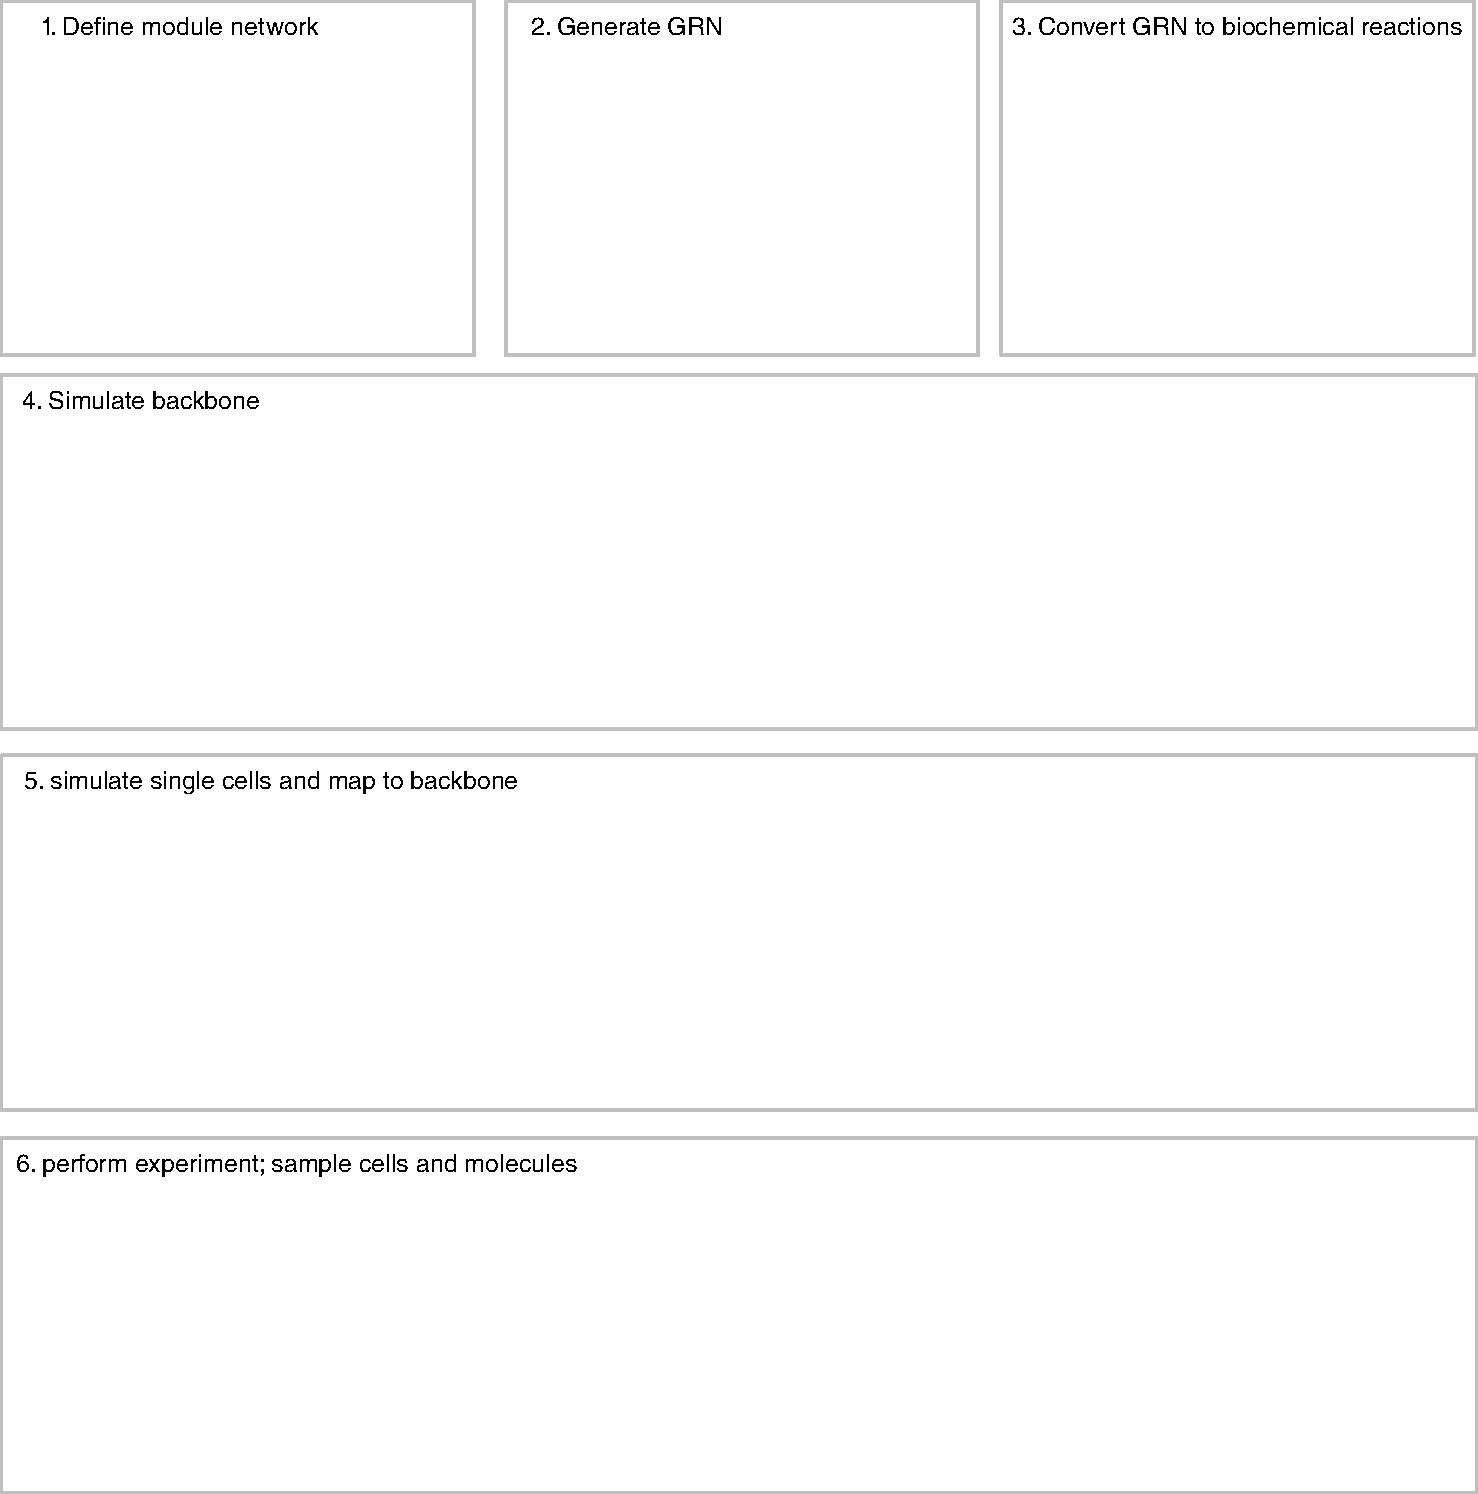
\includegraphics[width=\hugefigure]{fig/explain_methods} 
	\caption{\textbf{The workflow of dyngen is comprised of six main steps.} \textbf{A:} The user needs to specify the desired module network or use a predefined module network. \textbf{B:} Each gene in a module is is regulated by one or more transcription factors from the upstream module. Additional target genes are generated. \textbf{C:} Each gene regulatory interaction in the GRN is converted to a set of biochemical reactions. \textbf{D:} Along with the module network, the user also needs to specify the backbone structure of expected cell states. The average expression of each edge in the backbone is simulated by activating a restricted set of genes for each edge. \textbf{E:} Multiple Gillespie SSA simulations are run using the reactions defined in step C.  The counts of each of the mocules at each time step are extracted. Each time step is mapped to a point in the backbone. \textbf{F:} Multiple cells are sampled from each simulation. Molecules are sampled from each cell.}
	\label{fig:explain_methods}
\end{figure}

\subsection{Defining the module network and backbone}

One of the main processes involved in cellular dynamic processes is gene regulation, where regulatory cascades and feedback loops lead to progressive changes in expression and decision making. The exact way a cell chooses a certain path during its differentiation is still an active research field, although certain models have already emerged and been tested \textit{in vivo}. One driver of bifurcation seems to be mutual antagonism, where two genes \cite{xu_regulationbifurcatingcell_2015} strongly repress each other, forcing one of the two to become inactive \cite{graf_forcingcellschange_2009}. Such mutual antagonism can be modelled and simulated \cite{wang_quantifyingwaddingtonlandscape_2011, ferrell_bistabilitybifurcationswaddington_2012}. Although the two-gene model is simple and elegant, the reality is frequently more complex, with multiple genes (grouped into modules) repressing each other \cite{yosef_dynamicregulatorynetwork_2013}.

In dyngen, the user defines the behaviour of the simulation by defining how sets of genes, called modules, are regulating eachother.
A module may have basal expression, which means that pre-mRNA of the genes in this module will be transcribed without the presence of transcription factor molecules. A module marked as "active during the burn phase" means that this module will be allowed to generate expression of its genes during an initial warm-up phase (See section \ref{sec:dyngen_ssa}). At the end of the dyngen process, cells will not be sampled from the burn phase simulations.

Several examples of module networks are given (Figure \ref{fig:example_backbones}). 
A simple chain of modules (where one module upregulates the next) results in a \emph{linear} process. By having the last module repress the first module, the process becomes \emph{cyclic}. Two modules repressing eachother is the basis of a \emph{bifurcating} process, though several chains of modules have to be attached in order to achieve progression before and after the bifurcation process. Finally, a \emph{converging} process has a bifurcation occurring during the burn phase, after which any differences in module regulation is removed.

Note that these examples represent the bare minimum in terms of number of modules used. Using longer chains of modules is typically desired. In addition, the fate decisions made in this example of a bifurcation is reversible, meaning cells can be reprogrammed to go down a different differentiation path. If this effect is undesirable, more safeguards need to be put in place to prevent reprogramming from occurring (Section \ref{sec:dyngen_backbone_lego}).

\begin{figure}[htb!]
	\centering
	\includegraphics[width=\LARGEfigure]{fig/example_backbones} 
	\caption{Example module networks}
	\label{fig:example_backbones}
\end{figure}

In addition to the module network, the user also needs to define a network of cellular states called the "backbone". Before simulating any cells, each transition in the backbone is simulated separately to obtain the average changes in expression along that transition (Figure \ref{fig:explain_methods}D). As part of the backbone, the user needs to specify which modules are allowed to alter its expression from one state to another. For example, in order to transition from state S0 to S1 in the cyclic example, gene modules A, B and C are turned on and a simulation is allowed to run. To transition from S1 to S2, gene modules D and E are turned on, and expression of gene module C is kept constant. To transition from S2 to S3, C is turned on again and now A and B are fixed. Finally, to transition from S3 to S1 again, A and B are turned on again and D and E are fixed again. Demonstrations of the backbone will be explained in more detail in section \ref{sec:dyngen_sim_backbone}.

\subsubsection{Backbone lego} \label{sec:dyngen_backbone_lego}

\paragraph{Simple linear}

\paragraph{Linear flip flop}

\paragraph{Linear double repressing}

\paragraph{Linear quick double repressing}

\paragraph{Bifurcation (reversible)}

\paragraph{Bifurcation (irreversible)}

\subsubsection{Predefined backbones}

\paragraph{Linear}
\paragraph{Bifurcating}
\paragraph{Cycle}
\paragraph{Branching} (and binary tree, consecutive bifurcating, trifurcating)
\paragraph{Converging}
\paragraph{Bifurcating converging}
\paragraph{Bifurcating cycle}
\paragraph{Bifurcating loop}
\paragraph{Disconnected}


\subsection{Generate gene regulatory network}
\blindtext
\subsubsection{Generate the transcription factor network}
\blindtext
\subsubsection{Generate targets and housekeeping genes}
\blindtext

\subsection{Convert gene regulatory network to a set of reactions}
\blindtext

\subsection{Simulate developmental backbone} \label{sec:dyngen_sim_backbone}
\blindtext

\subsection{Simulate single cells} \label{sec:dyngen_ssa}
\blindtext

\subsubsection{Map SSA simulations to backbone}
\blindtext

\subsection{Simulate experiment}
\blindtext

\subsubsection{Snapshot experiment}
\blindtext

\subsubsection{Time series experiment}
\blindtext

\subsubsection{Perturbation experiment}
\blindtext

\subsection{Example use cases}
\subsubsection{Trajectory alignment}
From discussion: Adding batch effects to snapshot simulations of linear (or even branching) trajectories allows evaluating trajectory alignment methods -- which attempt to map two or more trajectories onto each other. 
\subsubsection{Differential network inference}
From discussion: Adding perturbations to the GRN allows evaluating the performance of differential network inference methods -- which predict differential regulatory interactions between two or more groups of profiles.
\subsubsection{RNA velocity}
From discussion: Sampling a cell at a certain time point and once more at a later time point allows evaluating the performance of RNA velocity approaches -- which predict the future state of a cell by looking at differences in pre-mRNA and mRNA abundance levels.







%dyntoy and PROSSTT are specifically developed to generate datasets
% containing single cells which develop along a certain trajectory.
% These generators start a certain topology in mind, 
% simulate changing gene expressions along each of the branches of the topology, and sample cells
% from random points in the trajectory. splatter is focused on well replicating the specific noise characteristics of
% scRNA-seq data, and simulates differentially expressed genes in order to replicate clusters of cells, batch effects
% and even trajectories. dyngen 1.0 borrows a page from GeneNetWeaver in that it also converts a GRN into an ODE, but
% the GRN is constructed in such a way that the repeated simulations resemble single cells following a regulatory program
% (e.g. differentiation into one of two celltypes). BoolODE uses the dyngen 1.0 GRNs but uses boolean models to convert 
% the network into an ODE, and is used to evaluate the performance of NI methods, not TI methods. 

%\begin{table}
%	\caption{\textbf{Comparison of existing single-cell omics simulators.} TI: trajectory inference, NI: network inference, Cl: clustering, DR: dimensionality reduction.} \label{tab:simulators}
%	\centering\fontsize{9}{11}\selectfont
%	\begin{tabularx}{\linewidth}{p{1.6cm}p{2.5cm}p{3cm}X}
%		Generator & Used to evaluate & Data type(s) & Approach \\ \hline
%		dyngen 1.0 & TI & mRNA \& protein & GRN, ODE, Euler--Maramuya \\
%		dyntoy & TI & mRNA & Visualise tree in plane, generate expression in plane, sample cells from tree \\
%		PROSSTT & TI & mRNA & Random walks along tree, sample cells from tree \\
%		splatter & Cl \& TI & mRNA & Simulate DE genes, simulate scRNA-seq noise \\
%		BoolODE & NI & mRNA \& protein & Use dyngen GRN's, ODE, Euler--Maramuya \\
%		dyngen 2.0 & TI, NI, Cl, DR & pre-mRNA, mRNA, protein & Backbone, GRN, SSA \\
%		dyngen 3? & TI, NI, Cl, DR & pre-mRNA, mRNA, miRNA, protein, protein complex & Backbone, GRN, SSA
%	\end{tabularx}
%\end{table}
